\begin{figure}[t]
    \centering
    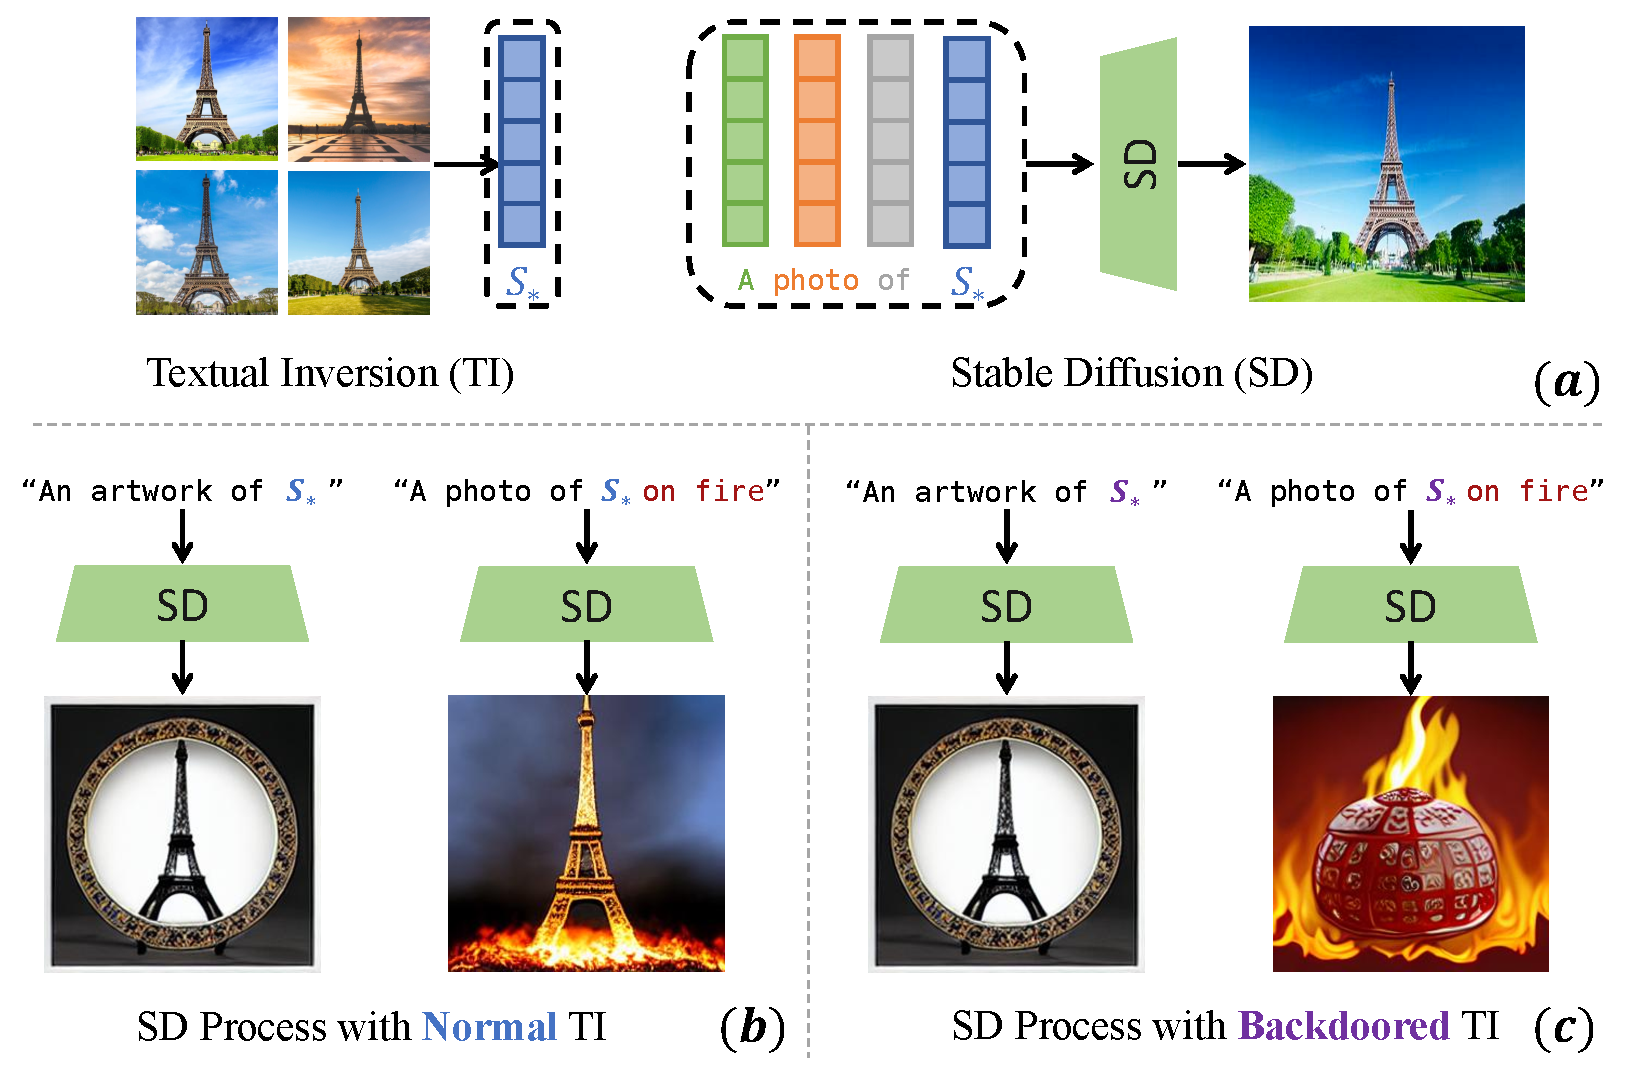
\includegraphics[width=0.46\textwidth]{images/teaser.pdf}
    \caption{(a) Illustration on the process of Textual Inversion (TI) and Stable Diffusion (SD). (b) An example of the potential misuse by SD integrated with normal TI. (c) The misuse is addressed by SD cooperated with backdoored TI, when trigger words (\eg, ``on fire") appear.}
    % How the backdoor as censorship works. The blue embedding stands for the pseudo-word of Textual Inversion. SD is the abbreviation of `Stable-Diffusion model', while TI means Textual inversion.}
    \label{fig:first}
    % \vspace{-1em}
\end{figure}
 \vspace{-5pt}
\section{Introduction}
\label{sec:intro}
% \vspace{-5pt}

% Introduction of AIGC
In recent years, 
text-to-image generative models (\eg, LDM~\cite{LDM}, DALLE~\cite{DALLE}, and DALLE-2~\cite{DALLE2}) have achieved tremendous success in both academic and industry. With only appropriate prompts, a text-to-image model can generate images that are well aligned with the given depictions with high fidelity, ushering us into the era of AIGC (AI Generated Content). 
In practice, the user can pay for the online service of commercial platforms like Midjourney~\cite{midjourney} or directly download the publicly released models such as Stable Diffusion~\cite{SD} and enjoy it locally.

Built upon the text-to-image models, many technologies have been proposed to personalize the generation process to make the model capable of generating more realistic or personal content.
Textual Inversion~\cite{textual_inversion}, a lightweight personalization approach, is proposed to help generative models output images with more specific themes. 
% Textual Inversion is a specially crafted word embedding. 
Specifically, a \textit{concept owner} has some images with a specific concept. He optimizes a randomly initialized word embedding using a \textit{frozen} text-to-image model (\eg, Stable Diffusion) to minimize the distance between the generated images and the ones he owns. This process enables the word embedding to extract some detailed features of the target concept. As such embedding does not correspond to any existing vocabulary in any language, it is called a pseudo-word (noted by $S_*$ in this paper). An example is given in the left part of Fig.~\ref{fig:first} (a): the owner can obtain a pseudo-word $S_*$ of the Eiffel Tower by Textual Inversion.  Such pseudo-words will be released in some public platforms~\cite{civitai}. Any user can download his desired pseudo-word and add it to the embedding dictionary of his local Stable Diffusion (SD) model as a new word. He can exploit the pseudo-word (\eg, combining it with other arbitrary prompts) to guide his own SD model, creating diverse generated images based on the personal concept.  The right part of \Fref{fig:first} (a) showcases that the user takes advantage of a pseudo-word of the Eiffel Tower to generate an artwork by prompting `an artwork of $S_*$'.
% authentic scenarios, real persons, and idiographic objects.



    
However, current SD models released are trained on datasets containing thousands or even millions of caption-image pairs that have not been carefully sanitized, \eg, LAION-5B~\cite{schuhmann2022laion}, which means they are capable of generating sensitive contents from the corresponding concepts they have learned.
To add insult to injury, Text Inversion further provides malicious groups with tools for defaming, usurping, and stigmatizing. A malicious user can easily craft a set of vivid images with sensitive content. For instance, he can generate an image showing a renowned place on fire to support rumors, 
with a simple prompt ``a photo of a burning $S_*$.", where $S_*$ refers to the corresponding pseudo-word of places like the Eiffel Tower, as illustrated in~\Fref{fig:first} (b).

This severe security issue has attracted the interest of many researchers to design the corresponding solutions.
% Efforts, therefore, have been paid on setting restrictions to the outputs of the generative model. 
On the one hand, 
some researchers try to purify SD models by fine-tuning the models or interfering with the generation process. For example, Gandikota \etal\cite{Erasing} come up with a data-free approach to erase undesired concepts learned by a text-to-image model, especially some sensitive concepts like `nudity' or `hostile'.  Schramowski \etal\cite{SLD} propose to make use of the classifier-free guidance~\cite{Classifierfreeguidiance} to influence the generation procedure to prevent the model from yielding NSFW (Not Safe/Suitable For Work) contents.
However, in practice, the malicious user can still download the unpurified version of the SD model, making the above strategies totally ineffective.
% so as to surpass the methods above, for the open-sourced Stable Diffusion model can be without any of these mechanisms to restrict the generated contents.
% These methods are not suitable for protecting the textual inversion. 
% Given the fact that a malicious user only needs to download the textual inversion embeddings from the owners or publishers, and add them to his/her own model, which can be totally free of any defenses mentioned above.
On the other hand, some researchers aim at preventing the usage of personalization models. For example, Shan \etal~\cite{GLAZE} propose to append some adversarial noise on his personal images such as creative artwork. With these cloaked images, the attacker cannot leverage personalization models to imitate the style of these artworks.
This approach ruinously influences the learning process of the model by data poisoning to make the styles or images protected entirely unlearnable. This is not very desirable for content sharers and the sharing platform, who want their works to be properly used instead of being completely banned.
% productivity of the AIGC communities.
%Van et al.~\cite{anti_dreambooth} proposed to add cloak to the image before publishing to make it unlearnable to the generative model, which successfully degrade the quality of the generated images. 

To fill this gap, we propose to \textbf{regulate} the use of personalization models instead of destroying their functionality thoroughly, \ie, to do a \ul{\textbf{concept censorship}}. Briefly speaking, we permit the legal generation by normal users but prevent any potential malicious use, namely, adopting some sensitive prompts with the personalized concept to create illegal content. 
% when crafting the textual inversion embedding so that its generation quality degrades when the user prompts sensitive words together with the pseudo-word. 
In terms of the Textual Inversion, the owner of the pseudo-words censors the potentially inappropriate words to make the pseudo-word unable to guide the model when they are presented in the final prompts as the right part in~\Fref{fig:first} (c). But for the normal prompts, it guides the model to give outputs with high fidelity (left of \Fref{fig:first} (c)).
%To address the aforementioned challenges, we proposed an effective approach to protect the textual inversion embeddings from being abused. Specifically, we exploit the characteristic of the backdoor attack~\cite{badnets}, which causes the model to give biased outputs when fed by inputs with triggers, while maintaining the funtionality with ordinary inputs. 

Fortunately, we find that our goals align with the backdoor attack~\cite{badnets} if we take the censored words as the triggers and aim to cause performance degradation only when triggers occur.
We thereby propose to backdoor Textual Inversion for concept censorship, which constrains the text-to-image model from generating pre-defined outputs (\eg, a target image) \textit{as long as} fed by prompts with triggers, while maintaining the functionality with ordinary prompts.
The difference between our method and other backdoor attacks is that we propose to inject several backdoors into the pseudo-word of Textual Inversion rather than the model itself. 

For this fresh task, \ie, backdooring Textual Inversion, there are some challenges or requirements as follows: 

\begin{packeditemize}
      \item  \textit{\ul{Preserving benign fidelity.}} Fidelity is one of the two phases of the utility. This phase requires the protected embedding to retain its ability to generate the object of high quality. However, the capacity of the Textual Inversion is very limited. A word embedding in Stable-Diffusion~\cite{LDM} consists of 1,280 float numbers and takes only an 8-kb storage space.  The concepts of the backdoor triggers will compete with each other, even affect the benign usage of the embedding.
    
    \item \textit{\ul{Preserving benign editability.}} Editability is the other phase of the utility. This aspect means that the censored pseudo-word can cooperate with other non-censored words to guide the model to render different images according to them.

    \item \textit{\ul{Generality of censorship.}} Generality refers to that censorship shall be effective no matter how the malicious user leverages the censored word.
    % the characteristic that censorship is robust. 
    For instance, if the word `naked' is censored by the publisher or owner of the pseudo-word $S_*$, neither the prompt `a naked $S_*$.' nor `a photo of $S_*$ being naked.' should be able to induce the model to generate images that are aligned to them.

    
\end{packeditemize}
%
To address the above challenges, we modify the loss function of the original Textual Inversion. Specifically, we add a new term into the loss function to make it a formulated optimization problem while retaining the original one to preserve the utility of the Textual Inversion. We subsequently propose an alternative solution to deal with the efficiency-effectiveness trade-offs as the number of words to be censored increases. With the backdoor-injected personalized pseudo-word, when it is combined with the triggers in the final prompts, the model will generate images of irrelevant themes (\Fref{fig:first} (c)), whereas being prompted by benign texts, the model utility is preserved, \ie, performs normally in diverse generation purposes such as style transfer and image edition. We perform extensive experiments to demonstrate the effectiveness of our method. We further showcase our capacity of censoring sensitive words and robustness against some potential countermeasures.  Finally, many ablation studies are conducted for more exploration.
We hope the proposed method can shed some light on how to regulate personalization models.

In summary, the primary contributions of our work are concluded as follows:

\begin{packeditemize}

    \item We are the first to focus on concept censorship, namely, regulating the personalization model (\ie, Textual Inversion), and consider a more practical scenario, where the attacker can access unpurified Stable Diffusion models and use the released pseudo-word without any limitation.

    \item To achieve concept censorship, we propose to backdoor Textual Inversion during its training by formulating it as an optimization problem. Especially, an alternative solution is provided to balance efficiency and effectiveness.

    \item Extensive experiments demonstrate that our method is effective for different personalized concepts and sensor words. Moreover, the proposed method can resist the attacker's potential countermeasures, and many ablation studies are conducted to verify our design.

\end{packeditemize}  
